\section{Results}

In December of 2013 a total of 10 Bq of CH$_3$T was injected into LUX and removed. A total 325,000 events were observed in the active volume of LUX. 140,000 events were collected in the fiducial volume at the nominal LUX electric field of 180 V/cm, while 4,500 fiducial events were collected in a special run at a reduced field of 100 V/cm. The S1 and S2 signals are corrected for spatial effects such as the light collection efficiency and the free electron lifetime with $^83m$Kr data as described in \cite{lux-reanalysis}. 

We interpret the data in terms of the combined energy model \cite{platzmann}, where the total energy of an event is directly proportional to the number of quanta produced (electrons pus scintillation photons):

\begin{displaymath}
E_{total} = W \cdot (n_{\gamma} + n_e )
\end{displaymath}

\noindent
We use a $W$ value of 13.7 eV/quanta \cite{Dahl}. In LUX $n_{\gamma}$ and $n_e$ are proportional to the S1 and S2 signals, with gain factors $g_1$ and $g_2$:

\begin{displaymath}
E_{total} = W \cdot (\frac{S1}{g_1} + \frac{S2}{g_2} )
\end{displaymath}

\noindent
where S1 and S2 have units of phe and $g_1$ and $g_2$ have units of phe per quanta. $g_1$ may be interpreted as the light collection efficiency times the average quantum efficiency of the PMT arrays, while $g_2$ is the electron extraction efficiency at the liquid-gas surface times the secondary scintillation gain factor and the PTM quantum efficiency. $g_1$ and $g_2$ are measured with line source data in LUX as described in Ref. \cite{lux-reanalysis, lux-prd}. We find values of $g_1$ = \gone and $g_2$ = \gtwo.

\begin{figure}[h!]\centering
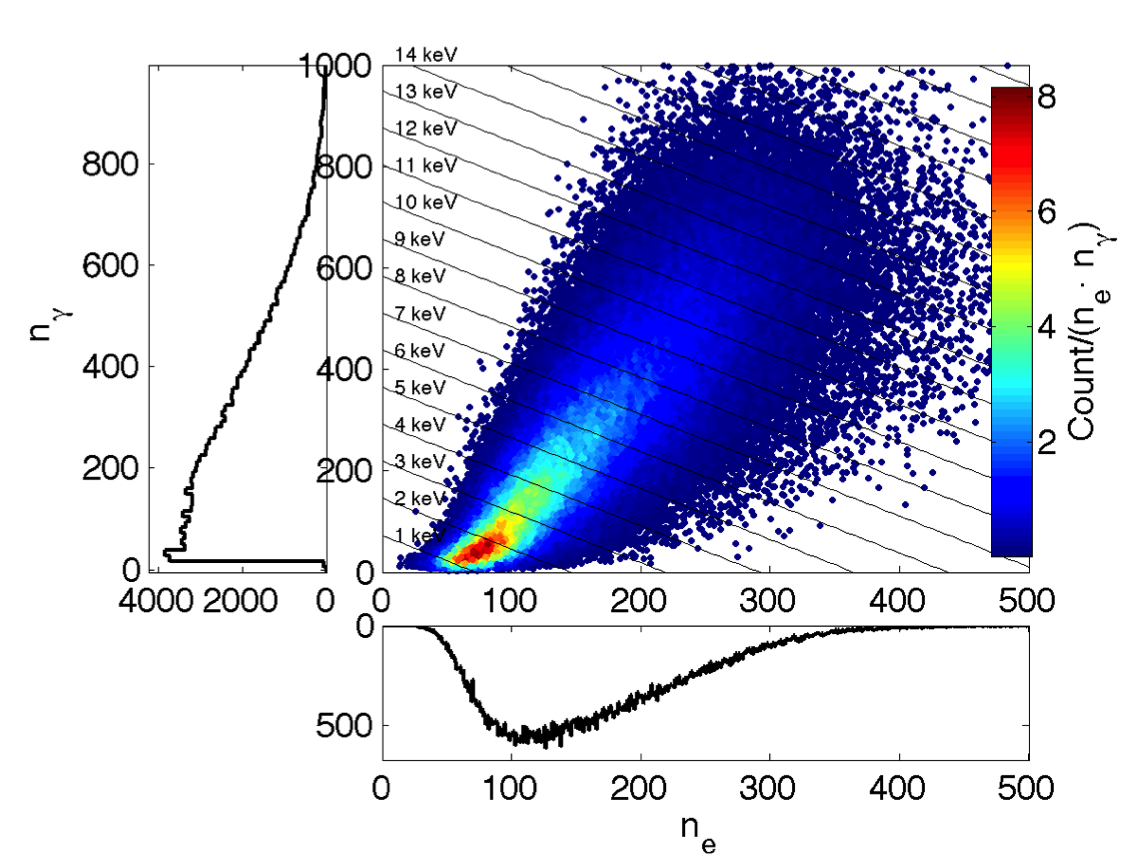
\includegraphics[width=90mm]{fig/tritium-scatter.png}
\caption{Scatter plot of $n_e$ vs $n_{\gamma}$ for 115,000 fiducial CH$_3$T events at 180 V/cm. Lines of constant energy are indicated assuming a $W$ value of 13.7 eV/quanta. The data is projected into $n_e$ and $n_{\gamma}$ histograms on each axis.}
\label{fig:tritium-scatter}
\end{figure}


\begin{figure}[h!]
\begin{center}
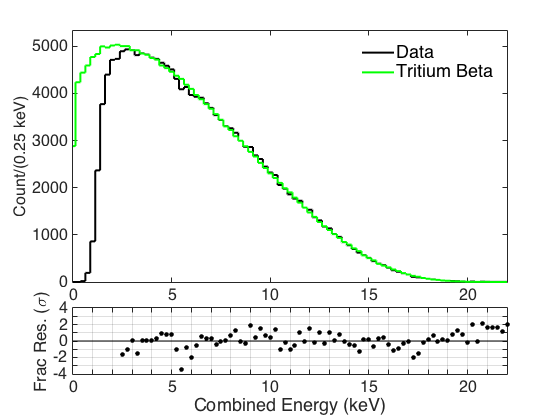
\includegraphics[width=90mm]{fig/tritium-spectrum-linear.png}
\caption{The CH$_3$T energy spectrum measured by LUX with the combined energy model (black) compared to several theory models: a pure tritium spectrum (dashed blue), LUXsim (red) and a tritium spectrum with a simple energy smearing of $\sigma_E = XXXX$ applied. }
\label{fig:tritium-spectrum}
\end{center}
\end{figure}



A scatter plot of $n_e$ vs $n_{\gamma}$ for the CH$_3$T data at 180 V/cm is shown in Fig. \ref{fig:tritium-scatter}, along with the projected histograms on each axis. The CH$_3$T energy spectrum, obtained by projecting the data along the lines of constant energy, is shown in Fig. \ref{fig:tritium-spectrum}. The data is compared to several models: a pure tritium spectrum, with no detector effects; a spectrum simulated with LUXsim, and a tritium spectrum with a simple energy smearing factor of $\sigma_E = XXXX$ applied. The ratio of the data to the smeared tritium spectrum is shown in Fig. \ref{fig:ER-threshold}, along with a fit to an error function. The ratio indicates that the data is well modeled by the smeared tritium spectrum, and the effective 50\% energy threshold is found to be 1.04 $\pm$ 0.016 keV. 

The comparison also illustrates the usefulness of the combined energy model. Compared to the raw charge and light spectra shown projected on the axes in Fig. \ref{fig:tritium-scatter}, the combined energy reproduces the tritium spectrum with much greater fidelity.

\begin{figure}[h!]\centering
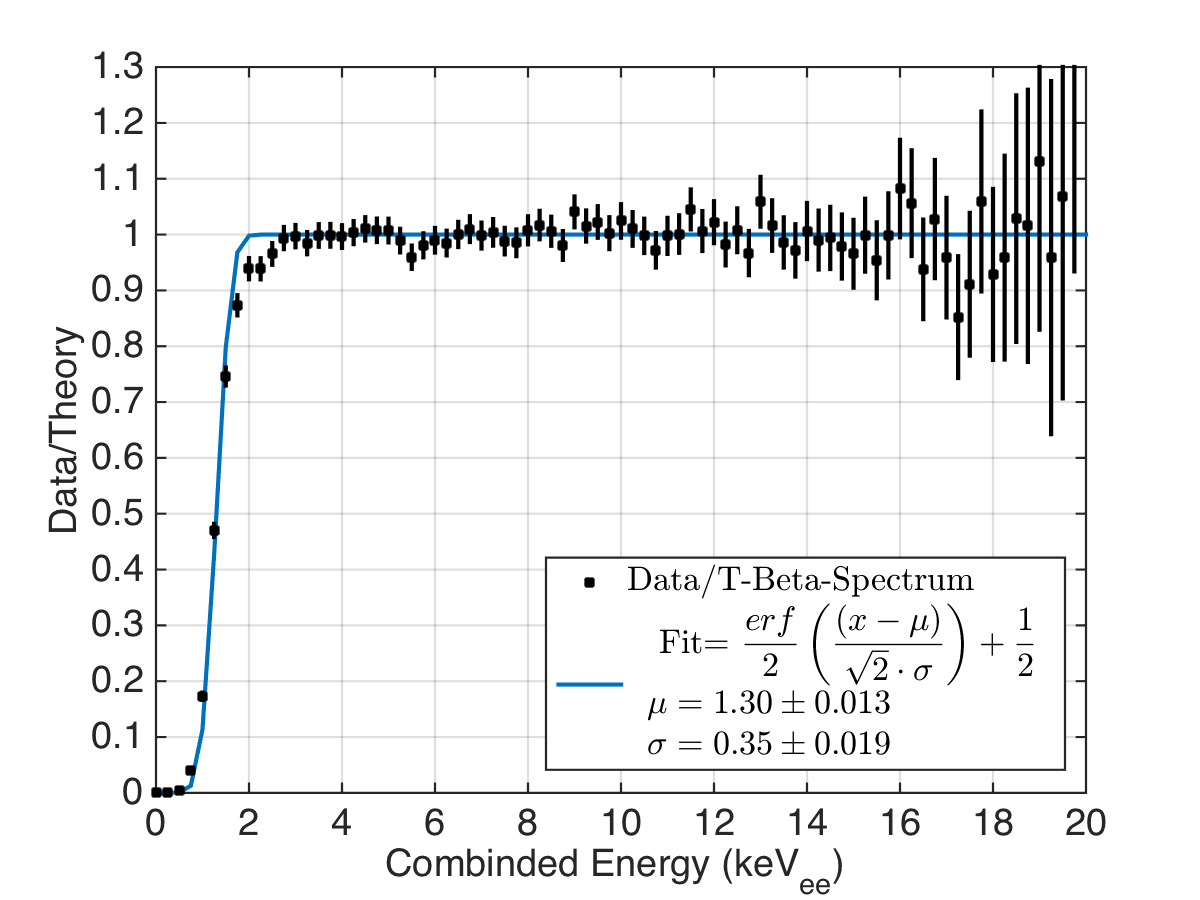
\includegraphics[width=90mm]{fig/E_Thres_Fit.png}
\caption{ER threshold measured by comparing the measured energy spectrum to the smeared tritium spectrum. A fit to an error function is shown.}
\label{fig:ER-threshold}
\end{figure}

The mean light yield and charge yield of ER events in LUX are obtained by dividing the mean light and charge signals by the combined energy in each energy bin. The result is shown for 180 V/cm in Fig. \ref{fig:ER-LY-QY}. For these plots a small correction has been applied to the data to account for smearing of tritium events across energy bins due to the detector's resolution \cite{attila-thesis}. 

\begin{figure}[h!]\centering
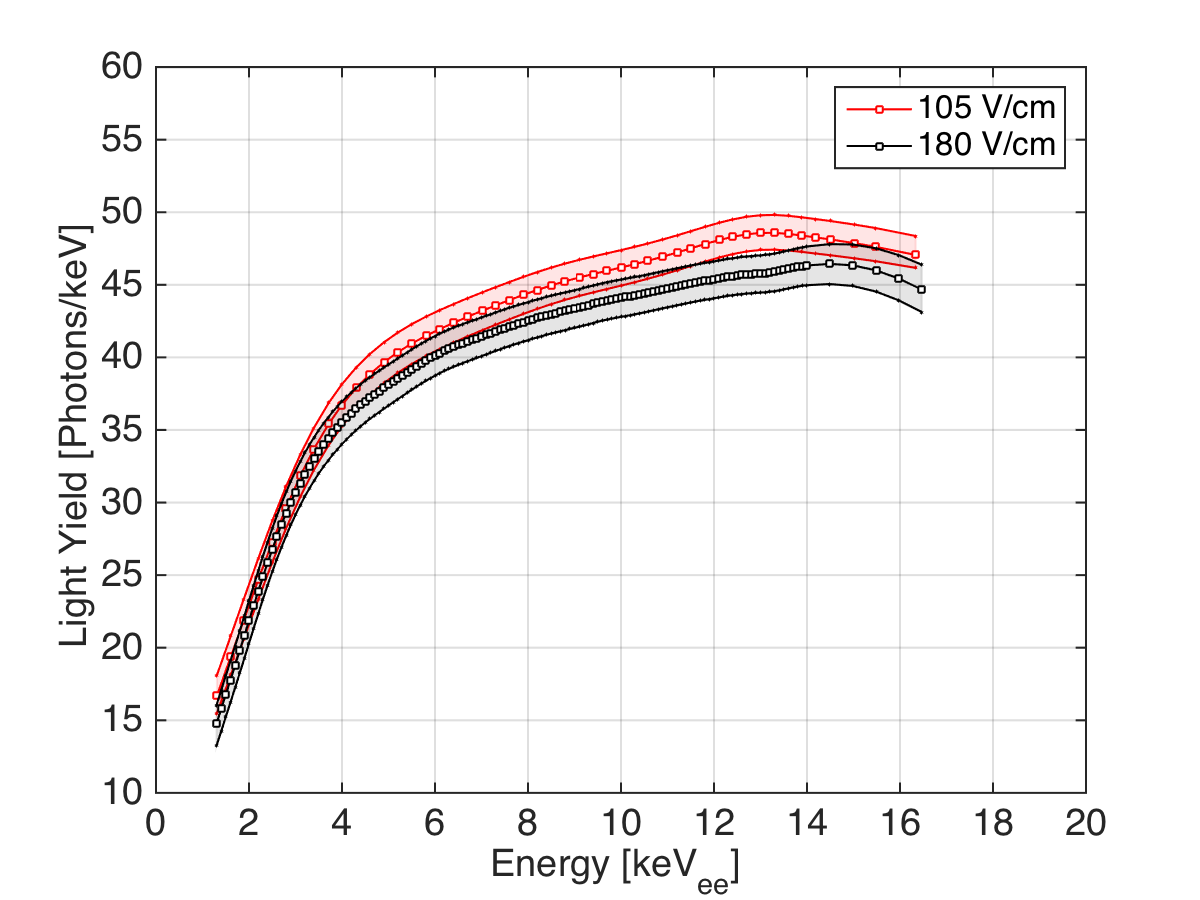
\includegraphics[width=90mm]{fig/ER_LY.png}
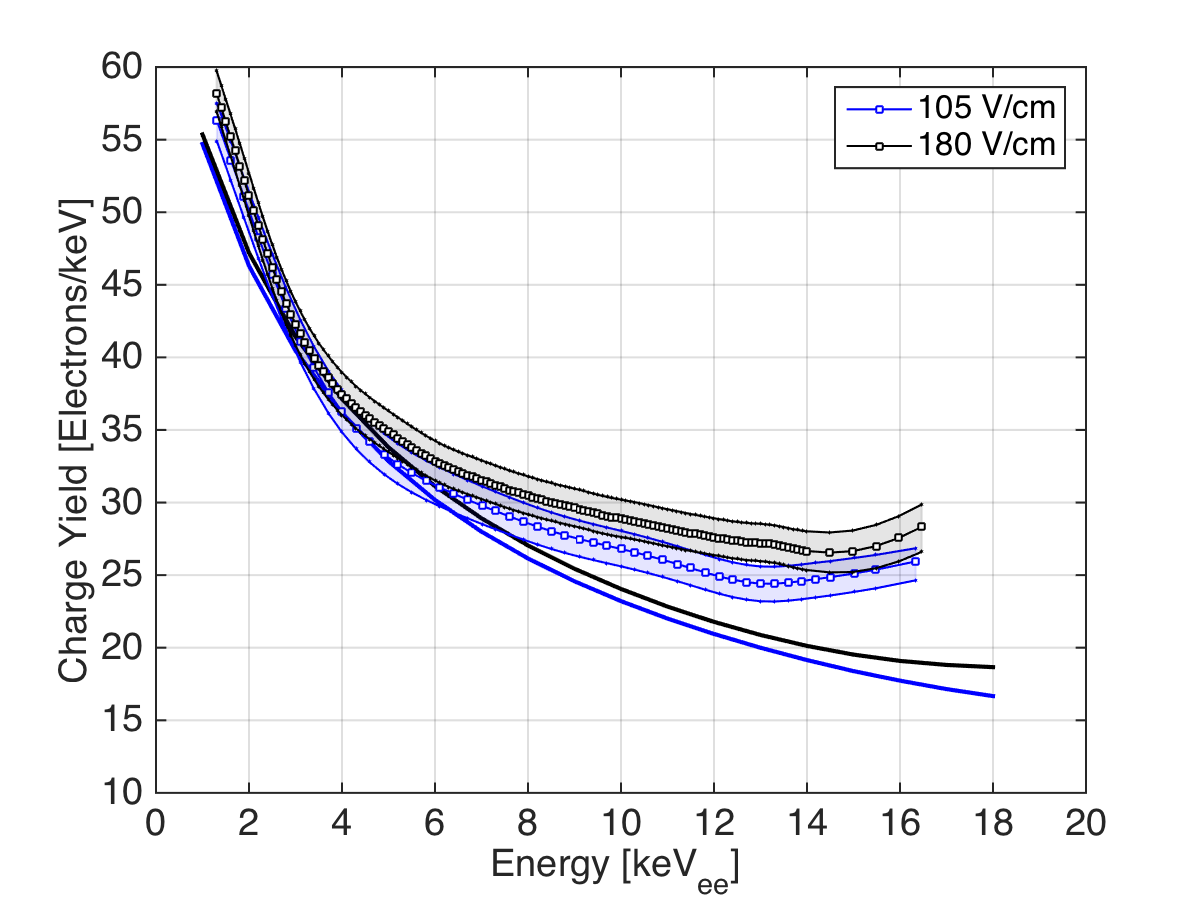
\includegraphics[width=90mm]{fig/ER_QY.png}
\caption{The light yield and charge yield of ER events in LUX at 180 V/cm compared to NEST v0.98 (2013). The grey bands indicate the systematic errors on $g_1$ and $g_2$, which are fully correlated across all energy bins. $g_1$ is anti-correlated with $g_2$, such that an increase in the charge yield within the grey band must be compensated by an equivalent decrease in the light yield. Upper: Light yield at 180 V/cm. Lower: the charge yield at 180 V/cm.}
\label{fig:ER-LY-QY}
\end{figure}

 \begin{figure}[h!]\centering
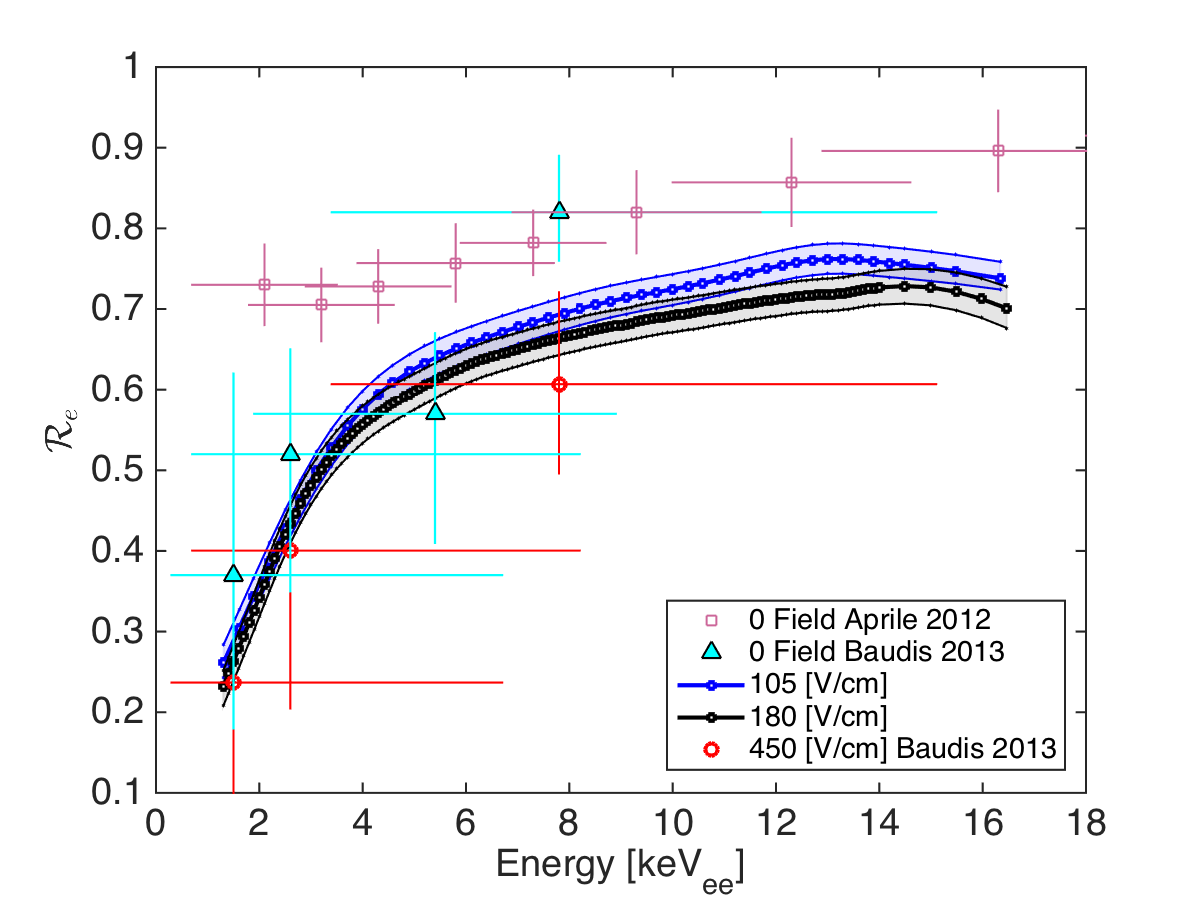
\includegraphics[width=100mm]{fig/Re_LY.png}
\caption{Scintillation yield relative to the yield of the 32.1 keV decay $\rm^{83}Kr $  vs. Energy. Shaded blue curve is tritium at 100 [V/cm], shaded black curve is tritium at 180 [V/cm], red circles represent a recent Compton scattering measurement at 450 [V/cm]. }
\label{fig:Re_LY}
\end{figure}


\begin{figure}[h!]\centering
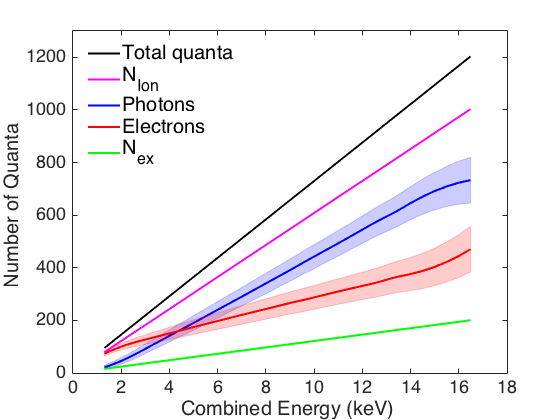
\includegraphics[width=90mm]{fig/quanta-vs-energy.png}
\caption{The mean number of electrons (red) and scintillation photons (blue) produced in LUX at 180 V/cm as a function of energy. The bands indicate the correlated systematic errors on $g_1$ and $g_2$. Also shown are the total number of quanta, primary ions, and primary excitons, assuming an exciton to ion ratio of 0.2. }
\label{fig:quanta-vs-energy}
\end{figure}


\begin{figure}[h!]\centering
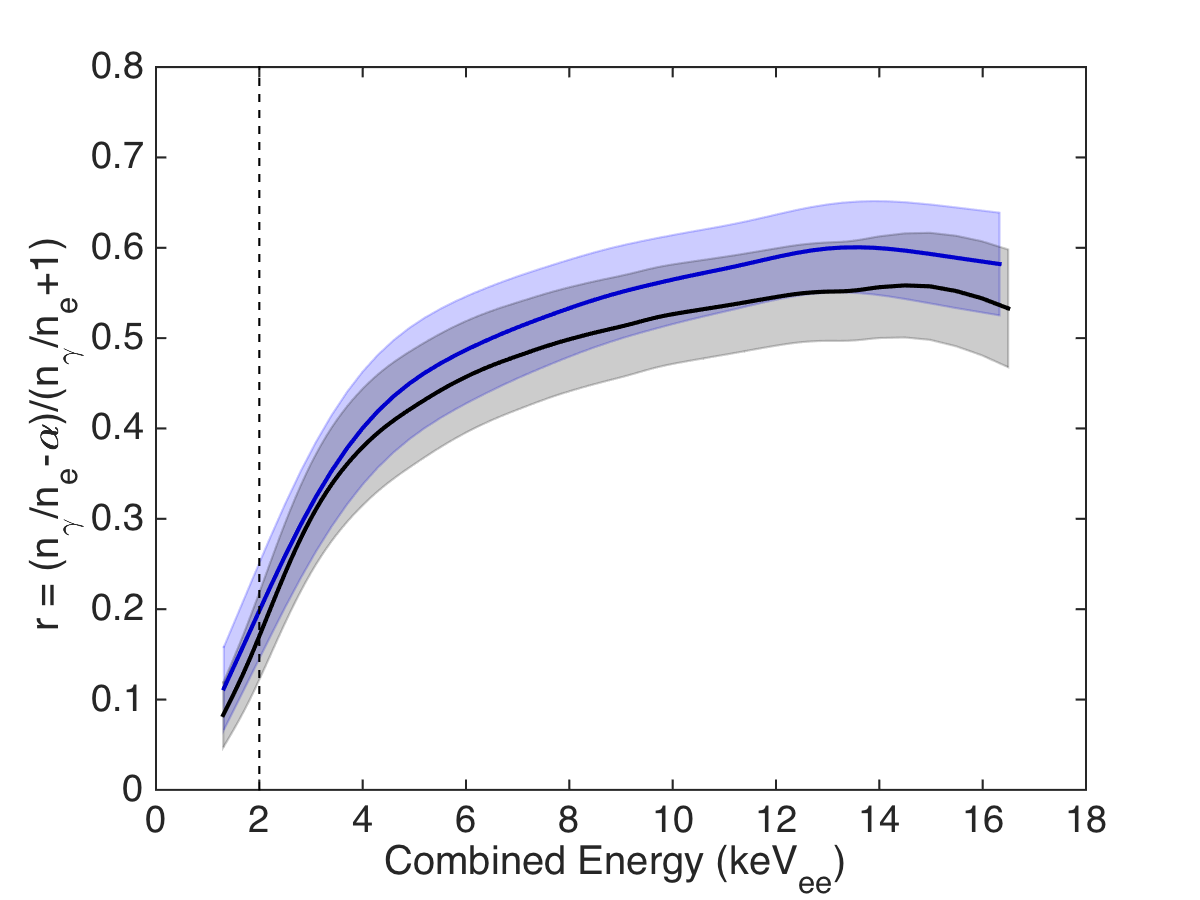
\includegraphics[width=90mm]{fig/recombination.png}
\caption{Recombination fraction of ER events at 180 V/cm, assuming an exciton-to-ion ratio of 0.2.}
\label{fig:recombination}
\end{figure}


As shown in Fig. \ref{fig:ER-LY-QY}, the light yield is observed to drop rapidly between 1 and 6 keV, and then become mostly energy independent over the remainder of the CH$_3$T spectrum. The charge yield exhibits the reverse behavior, as expected from the combined energy model. These effects can also be illustrated by plotting the total number of quanta as a function of energy, as shown in Fig. \ref{fig:quanta-vs-energy} for CH$_3$T events between 1 and 8 keV. Also shown in Fig. \ref{fig:quanta-vs-energy} are the total number of quanta assuming a $W$ value of 13.7 eV/quanta (black), and the primary number of ions (violet) and excitons (cyan) prior to recombination assuming an initial exciton-to-ion ratio of 0.2 \cite{XXXX}. In a model where the number of observed electrons differs from the number of primary ions due solely to recombination, we can interpret the charge yield data as a measure the recombination fraction at each energy. Accordingly, 

\begin{displaymath}
r = \frac{\frac{n_{\gamma}}{n_e} - \alpha}{\frac{n_{\gamma}}{n_e} + 1}
\end{displaymath}

\noindent
where $r$ is the recombination fraction and $\alpha$ is the assumed value of the primary exciton-to-ion ratio. Taking $\alpha = 0.2$, we find the recombination fraction as a function of energy as shown in Fig. \ref{fig:recombination}. Here the falling charge yield and rising light yield between 1 and 6 keV is interpreted as a rapid rise in the recombination fraction. 


\begin{figure}[h!]\centering
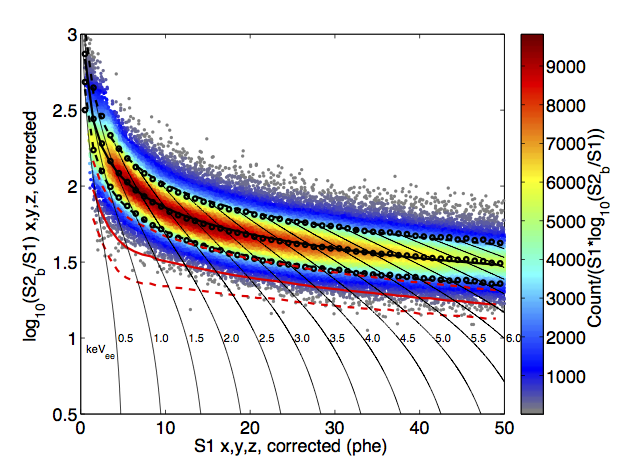
\includegraphics[width=100mm]{fig/CH3T_fid_50_2_Dec_Tritium_Approval_Plots.png}
\caption{The electron recoil band of LUX illuminated by 115,000 tritium events at the nominal LUX electric field of 180 V/cm.  The recoil discriminant variable, log(S2/S1), is shown vs. S1 between 1 and 50 phe in S1 (about $\rm1-8 keV_{ee}$). Also indicated in black are the mean and the 10\% and 90\% contours. The solid red line represents the mean NR band determined with NEST v0.98 (2013) \cite{nest} and validated with AmBe and $\rm^{252}Cf$ neutron sources and the DD neutron generator data. The dashed red indicates the 10\% and 90\% contours of the NR band.}
\label{fig:ER_band}
\end{figure}

We obtain the LUX ER band by plotting log$_{10}$(S2/S1) vs S1 as shown in Fig. \ref{fig:ER_band}. Also shown is the LUX NR band determined with NEST v0.98 (2013) \cite{nest} and validated with AmBe and $\rm^{252}Cf$ neutron sources and DD neutron generator data. The ER band has a characteristic rise at low S1 which reflects the increasing charge yield and decreasing light yield below 4 keVee, as seen in Fig. \ref{fig:quanty-vs-energy}. The leakage fraction ($f$), defined as the fraction of ER events that fall below the mean of the NR band, is shown in Fig. \ref{fig:Leak} as a function of S1. The recoil discrimination ($1-f$) has an average value of \fixit{99.58\%} for events with S1 between 1 and 30 phe.


\begin{figure}[h!]\centering
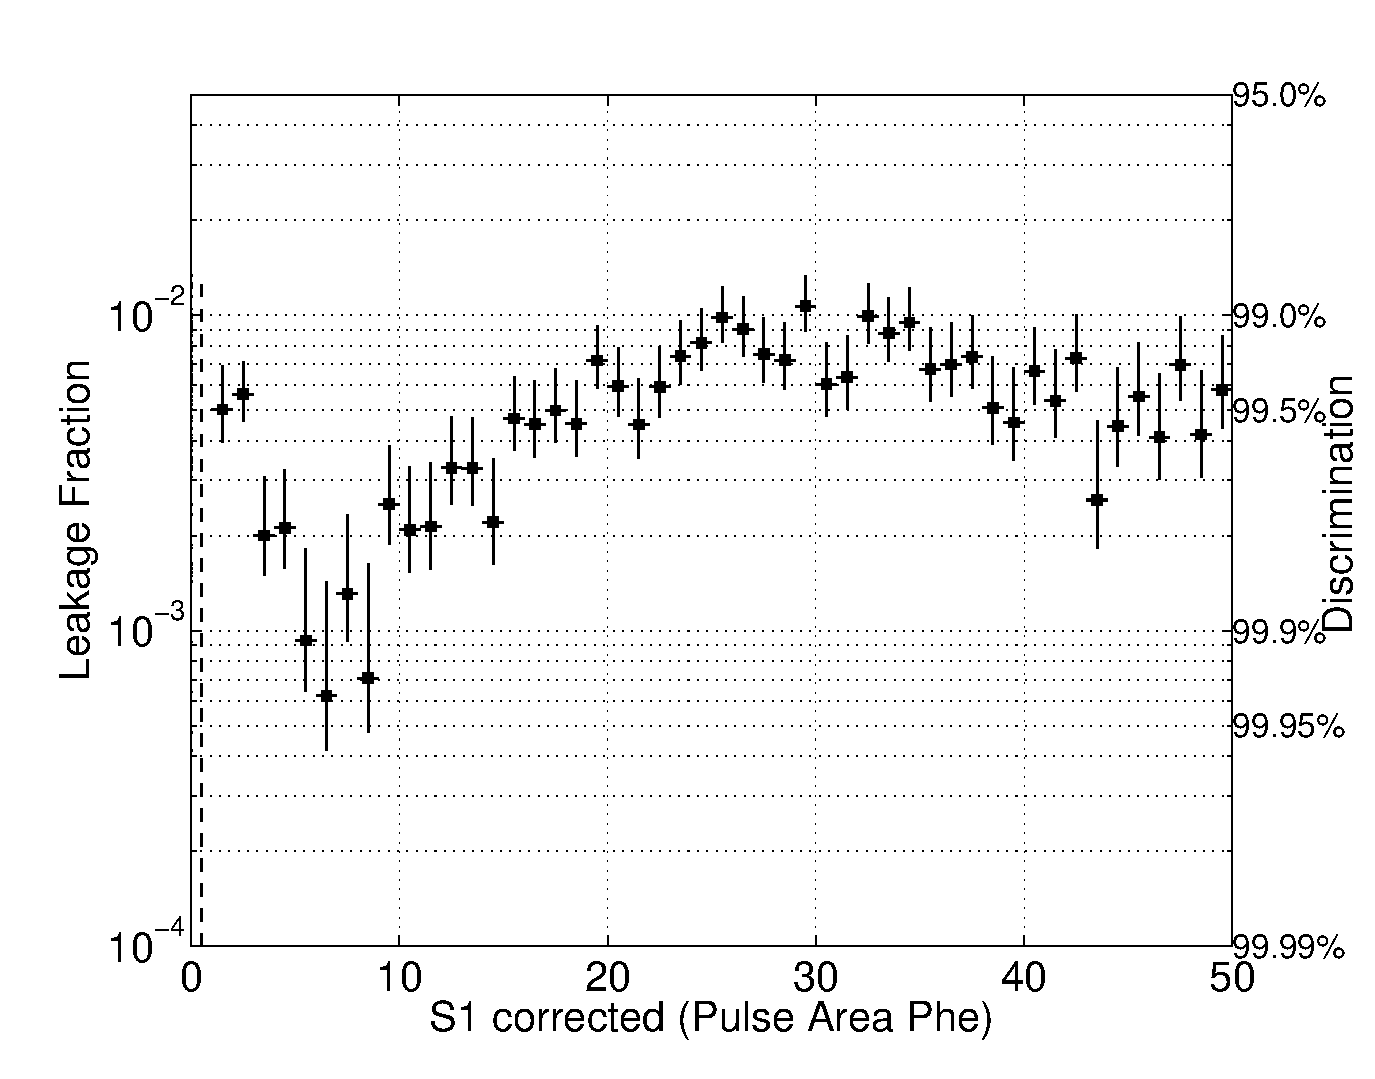
\includegraphics[width=90mm]{fig/CH3T_Leakage_fid_50_Dec_Tritium_Approval_Plots_2.eps}
\caption{LUX recoil discrimination vs. S1, determined from Fig. \ref{fig:ER_band}. Y-axis labels: left -  leakage fraction ($f$); right - discrimination ($1-f$).}
\label{fig:Leak}
\end{figure}


Figure \ref{fig:Spectrum} shows the reconstructed energy spectrum for those CH$_3$T events in the fiducial volume of the detector (black) along with the tritium spectrum from NEST modeling (blue) and an ideal tritium spectrum (magenta). The reconstructed energy matches the tritium beta spectrum well from 1 to 18 $\rm keV_{ee}$.
The calibration data was acquired in a 40 hour time window in which less than three out of 115,000 events are expected to be non CH$_3$T \cite{LUX_BG}, this implies a near perfect data purity for the calibration. Nearly every point (99.997\%) show in figure \ref{fig:Band} and the histogram of \ref{fig:Spectrum} is the result of a CH$_3$T beta decay in the fiducial volume of the LUX detector.

\begin{figure}[h!]\centering
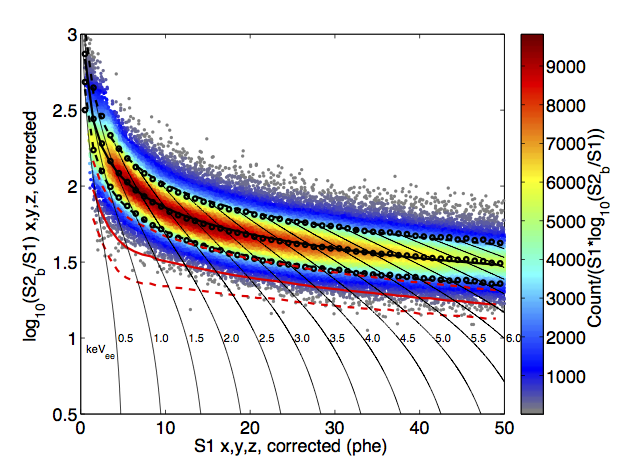
\includegraphics[width=100mm]{fig/CH3T_fid_50_2_Dec_Tritium_Approval_Plots.png}
\caption{Discrimination vs. S1 using over 115,000 tritium beta decays between 1 and 50 Phe in S1 (about $\rm1-8 keV_{ee}$). On average from 1 to 30 Phe the discrimination is 99.58\%, defined by the fraction of events of events below the mean of the nuclear recoil band. The red band represents the NEST nuclear recoil band (version 0.98) vetted with an AmBe, $\rm^{252}Cf$ and DD neutron generator calibration.}
\label{fig:Band}
\end{figure}


\begin{figure}[h!]\centering
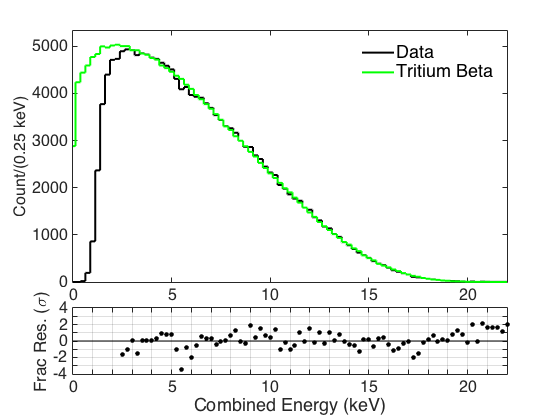
\includegraphics[width=100mm]{fig/tritium-spectrum-linear.png}
\caption{ Energy histogram of CH$_3$T events. The black histogram represents the data, in blue is the tritium spectrum produced with LUX SIM based on NEST. The magenta curve shows the true tritium beta spectrum without smearing due to finite detector resolution, the dashed line indicates the true tritium spectrum convolved with the threshold}
\label{fig:Spectrum}
\end{figure}


%Figure \ref{fig:NEST_v_Data} shows the comparison between simulation(NEST) and the data for the ER band. The agreement between simulation and data is good down to 7 Phe in S1. This is expected since at sub 2 $\rm keV{ee}$ (7 Phe in S1) data is limited and the NEST model has yet to be vetted at such low energies[Matthew/ Erik Dahl Thesis]. The newly acquired ER data below 2 $\rm keV{ee}$ from tritium will be used improve upon the NEST model at the extration field of 180 V/cm [ref?].

\begin{comment}

\begin{figure}[h!]\centering
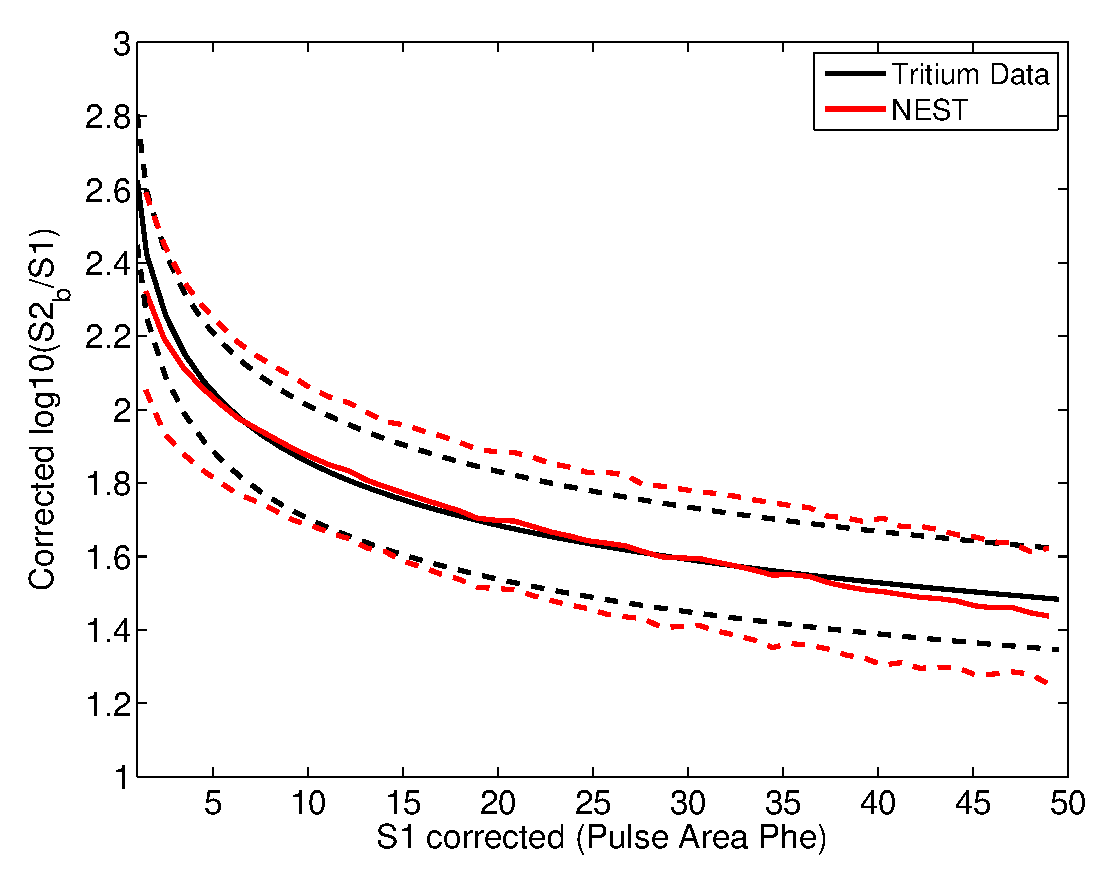
\includegraphics[width=80mm]{fig/CH3T_DATA_NEST_fid_30_LUX_SIM_Tritium.eps}
\caption{ER band measured using CH$_3$T data in black with 90\% confidence bounds ( $\rm \pm 1.3 \sigma$) compared with the NEST prediction in red.}
\label{fig:NEST_v_Data}
\end{figure}
\end{comment}

%%%%%%%%%%%%%%%%%%%%%%%%%%%%%%%%%%%%%%%%%%%%%%%%%


\subsection{Threshold Determination}

The CH$_3$T calibration source provides beta decays with energies down to 0.1 $\rm keV_{ee}$ allowing for an independent measure the LUX detector's threshold. The limitation for detecting a single scatter WIMP like event event with PMTs is the S1 (primary scintillation) signal, being more than an order of magnitude less than the S2 signal. The S1 threshold could be measured by comparing the NEST model, assuming perfect detector resolution, to the observed CH$_3$T beta spectrum from 0.1-10 $\rm keV_{ee}$. The threshold determined by comparing the CH$_3$T data to NEST is in good agreement with all other methods used for determining the threshold in the LUX detector, figure \ref{fig:S1_Thresh}. 

%The threshold for the S2 (bottom PMT array) shown is entirely due to the S1 threshold. We use only the bottom PMT array for the S2 signal because the secondary scintillation light is more uniformly distributed along the bottom PMTs than the top PMTs. 
%Figure \ref{fig:E_spec} shows the tritium beta spectrum measured in the LUX detector along with the NEST prediction, note at the 180 V/cm drift field NEST has been vetted form 2 to 10 $\rm keV{ee}$.

\begin{figure}[h!]\centering
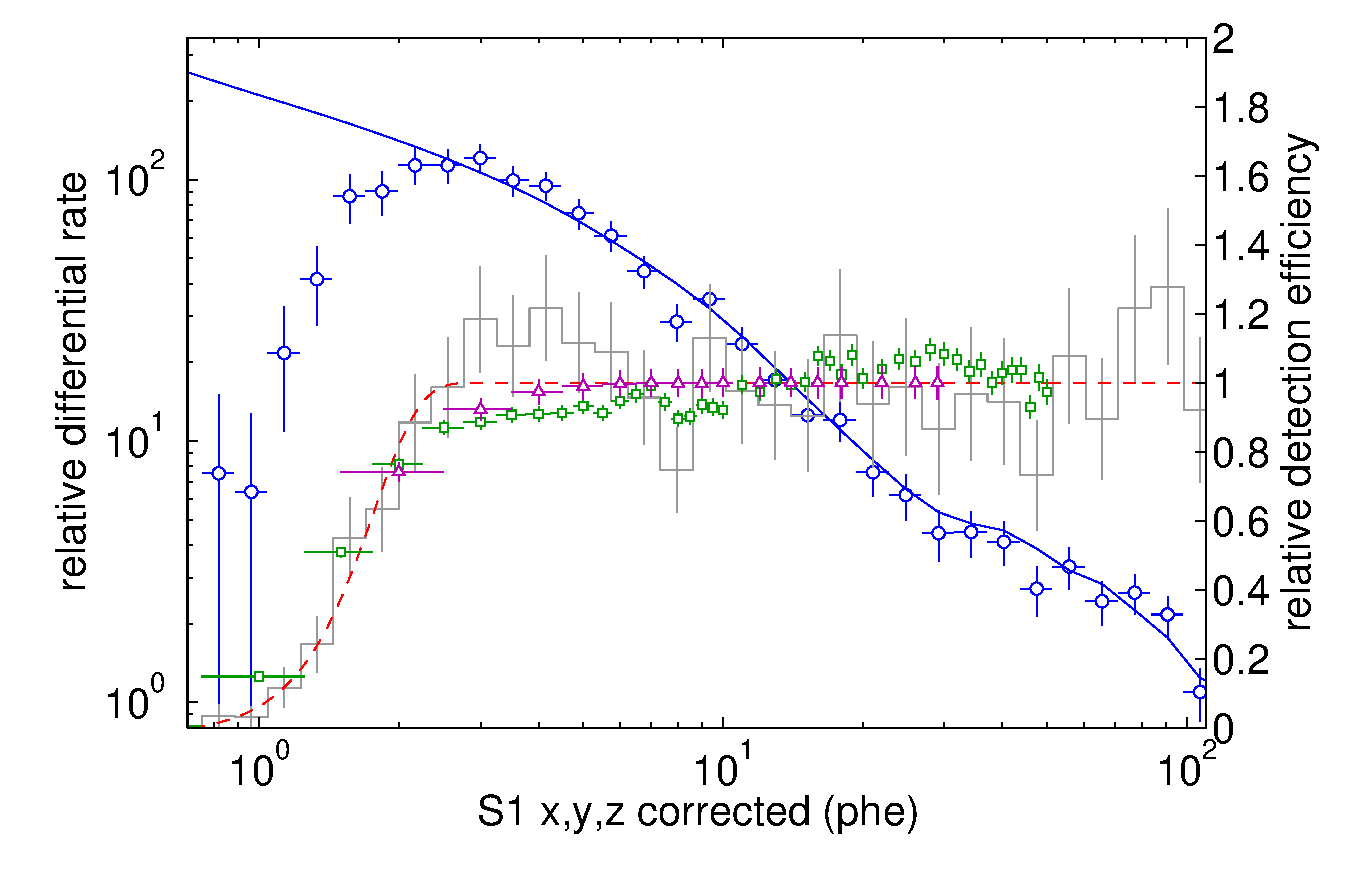
\includegraphics[width=100mm]{fig/Triritium_S1_Threshold_2013_PRL.eps}
\caption{Comparison of AmBe data (blue circles) with NEST simulations (blue line), showing excellent agreement above the 2 phe threshold (left axis). The gray histogram and fitted dashed red line show the relative efficiency for detection of nuclear recoils from AmBe data (right axis). Overlaid are the ER detection efficiency from CH$_3$T data (green squares), applied to the ER background model in the profile likelihood analysis, and the efficiency from full detector NR simulations treated as real data in terms of the digitized MC-truth S1 phe (purple triangles), applied to the WIMP signal model. The efficiency calculation here does not include S1 or S2 area thresholds. }
\label{fig:S1_Thresh}
\end{figure}


\begin{comment}

\begin{figure}[h!]\centering
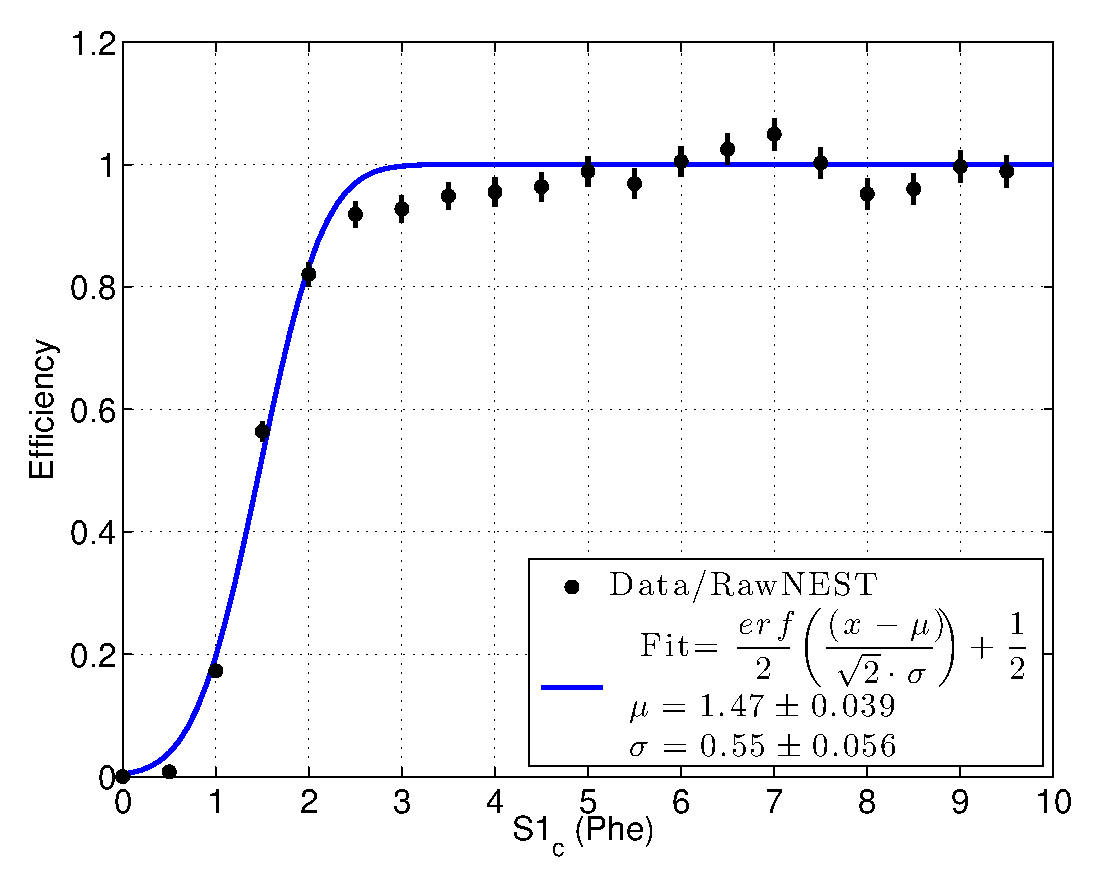
\includegraphics[width=80mm]{fig/CH3T_eff_S1_100_T_paper_corr_threshold.eps}
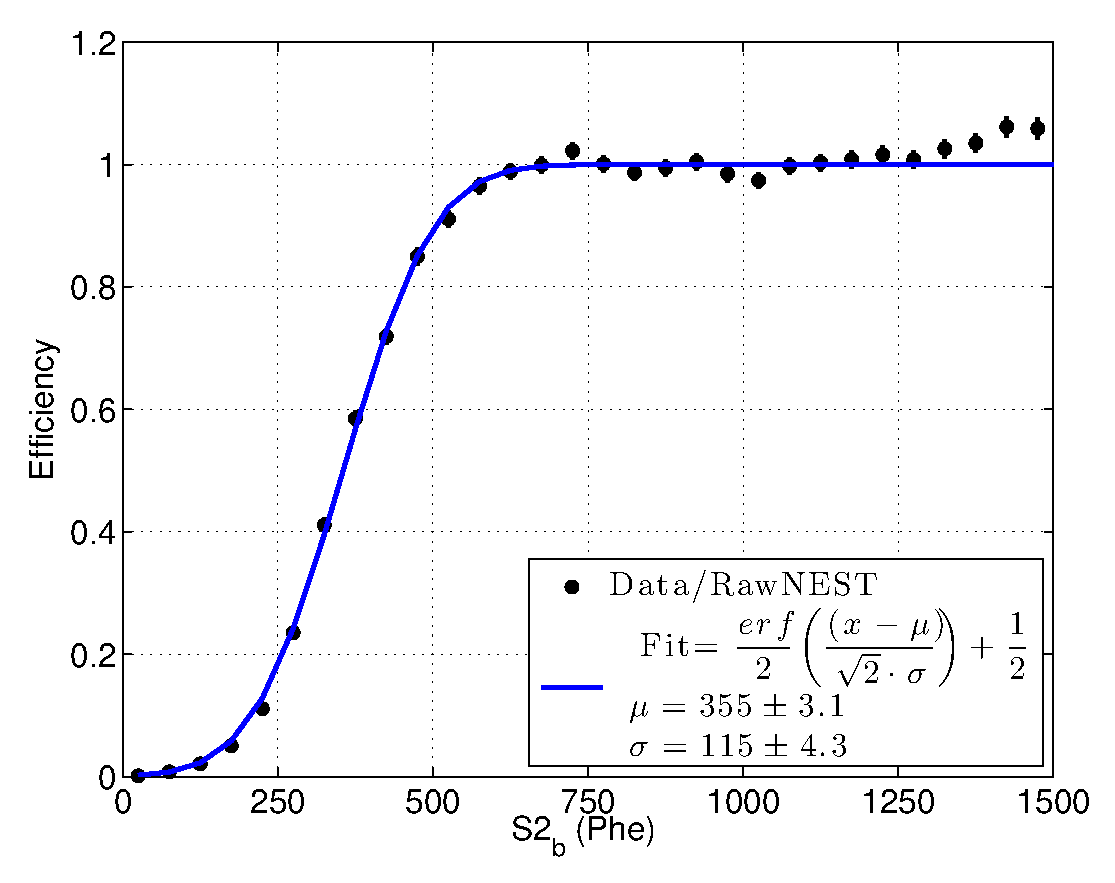
\includegraphics[width=80mm]{fig/CH3T_eff_S2_100_T_paper_corr_threshold.eps}
\caption{S1 Threshold determined from Tritium. S2 Threshold determined from CH$_3$T.}
\label{fig:S1S2_Thresh}
\end{figure}



\begin{figure}[h!]\centering
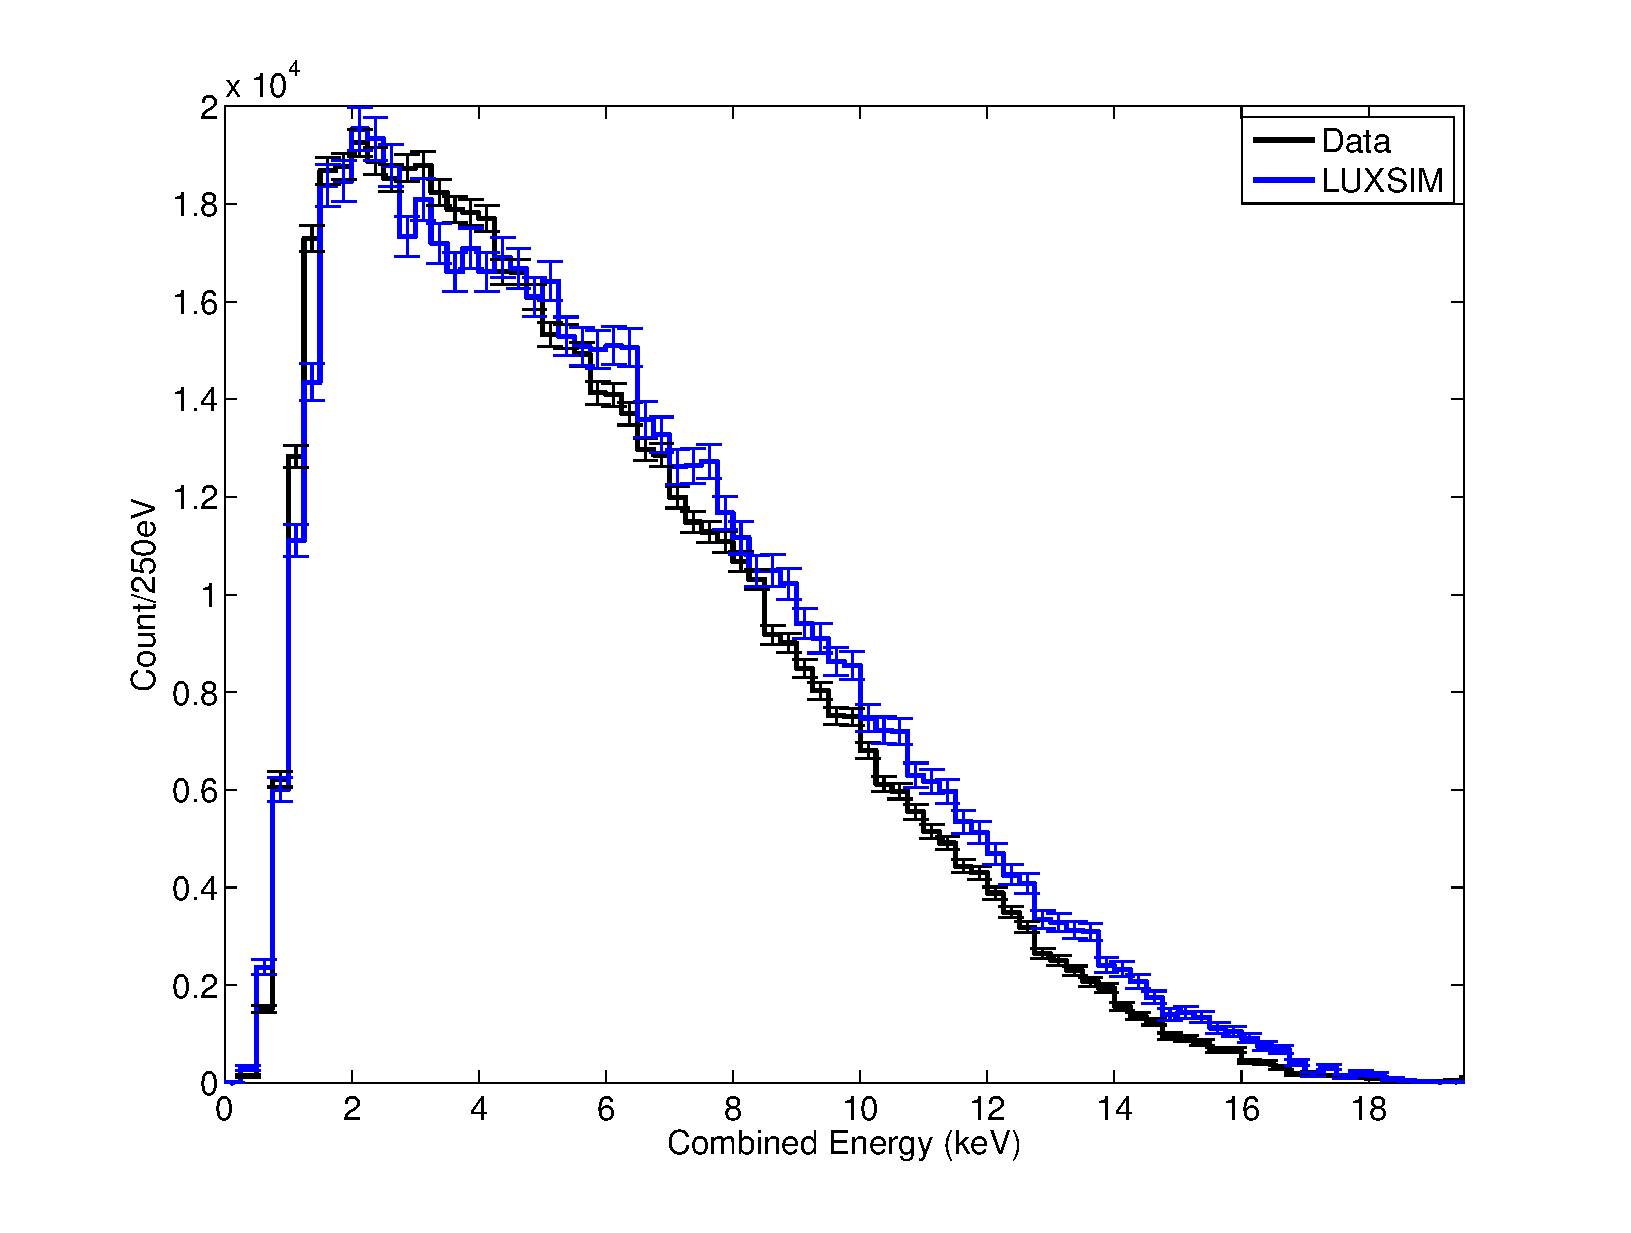
\includegraphics[width=100mm]{fig/CH3T_E_spec_18_Tritium_Dec_2013_180.eps}
\caption{Combined energy spectrum of the CH$_3$T data and LUX SIM.}
\label{fig:E_spec}
\end{figure}
 


 
 \subsection{Absolute Rate}
The absolute efficiency for detecting CH$_3$T events can be determined by comparing the number of observed events to the number expected. The initial activity injected was calculated to be $0.84 \pm 0.22 $ Bq, with the largest uncertainty coming from the ratio of $\rm CH_3T/CH_4$ from the CH$_3$T source bottle. The purification time constant was measured to be 6.6 hours. From the initial rate and the purification constant we expect to count a total of $20,200 \pm 4,000 $ events in the LUX detector before applying the S1 threshold. With the S1 threshold we expect  $16,000 \pm 3,100 $ `golden' events. The actual count observed in the liquid xenon volume was 20,000 events, which is in good agreement with the expected value taking into account the uncertainty in the initial activity and the purification model. After making fiducial cut $7,700 \pm  1,500$ events were expected and a total of $9,500 \pm 100$ were observed.
%,  roughly $16,000 \pm  3,100 * (290/324)*(18^2/24.5^2)$. 



\section{Scintillation Yield and Ionization Yield from Tritium Beta Decay}


\subsection{Cuts used in this analysis}
\begin{itemize}
\item Standard LUX Pulse finder classifier used in the WIMP search.
\item $\rm S2_b > 100 [Phe] $
\item PDE (g1) = 0.138 $\rm \pm 0.005$, measured with CH$_3$T
\item Extraction = 0.664 $\rm \pm 0.04$ measured with CH$_3$T.
\item single e- = 9.95 $\rm \pm 0.1$ [Phe/e-]
\item Using NEST 4c bands.
\end{itemize}




Scintillation and ionization yield are measured using the tritiated methane calibration source from the S1, S2 and reconstructed energy of each beta decay. The energy of each decay is determined using a prescription described in [Erik Dahl], see equations \ref{eq:Gain} and \ref{eq:E_comb}. 
\begin{equation}
\begin{split}
\rm  n_\gamma = \frac{S1}{g1}\\
\rm n_{e^{-}} = \frac{S2}{g2}
\label{eq:Gain}
\end{split}
\end{equation}

\begin{equation}
\begin{split}
\rm E= \frac{1}{W}(n_\gamma + n_{e^-})\\
\rm E= \frac{1}{W}(\frac{S1}{g1} + \frac{S2}{g2})
\label{eq:E_comb}
\end{split}
\end{equation}

The values of the work function W and gains g1, g2 have been measured using other calibration sources and are energy independent [ref]. Using equations \ref{eq:Gain} and \ref{eq:E_comb} we calculate the number of photons and electrons along with the energy of each tritium beta decay event to determine the yields. Scintillation and ionization yield are defined as [Photons/keV] and [Electrons/keV] respectively and the tritiated methane calibration source provides betas ranging from $\rm>1$ to 18 keV, with an exponential decline in event rate above 5 keV. For the results shown in figure \ref{fig:L_Q_Yield_180} over 150,000 beta decays in the fiducial volume were used to measure scintillation and ionization yield at 180 [V/cm]. A correction was applied for the beta spectral shape and the finite resolution of S1, S2 when measuring ionization and scintillation yield, the correction was found to be less than 10\% and is described in [my thesis]. Figure \ref{fig:L_Q_Yield_180} also shows the comparison of the results with the NEST model which has been vetted between 2 and 10 $\rm keV{ee}$. Also show are the measurements of light yield from a $\rm^{83m}Kr$ source, the 32.1 keV decay from $\rm^{83m}Kr$ is typically used as a standard calibration. (The second 9.4 keV decay from $\rm^{83m}Kr$  shown in the figure is for decays that occur more than 1000 ns after the initial 32.1 keV decay).

We find good agreement with the NEST model in the regions that have been vetted (2-10 $\rm keV{ee}$), see figure \ref{fig:L_Q_Yield_180}. Below 2 $\rm keV{ee}$ the light yield is lower than predicted by NEST and the charge yield is higher. The discrepancy between the data and the NEST model above 10 $\rm keV{ee}$ is due to limited data available for the model and also due to the track lengths of betas and gammas beginning to deviate above this energy. Note, under 10 $\rm keV{ee}$ track lengths of betas gammas are nearly identical. 

Figure \ref{fig:L_Q_Yield_Baudis} includes our light and charge yield measurements at 100 and 180 V/cm along with the recent Compton scattering measurement down to 1.5 $\rm keV{ee}$ from \cite{Baudis} at 450 V/cm. The error bars show in the figure include uncertainties from W, g1, g2 and the spectral shape correction. Unlike the measurement made using Compton scattering we can reconstruct energy using both the light and charge channels for each decay allowing for a powerful calibration down to 1 $\rm keV{ee}$ (corresponding to 80\% threshold at 2 Phe in S1).  We find a lower light yield than the centroids of the measurements in [ref Budias], however the the measurement is within reported errors. At our lower fields a higher light yield is expected than that measured at 450 V/cm due to less free charge separation.  The light yield of the 32.1 keV gamma from $\rm^{83m}Kr$ is shown on the figure as a measure of systematic uncertainty between the experiments. For the case of the standardized $\rm^{83m}Kr$ calibration source we find the expected behavior between the two experiments, a higher extraction field leads to lower light yield.

%\begin{figure}[h!]\centering
%\includegraphics[width=120mm]{LY_c_180_Tritium_Dec_2013_Charge_Yield_180_corr.png}
%\includegraphics[width=120mm]{CH3T_fid_E_S2_c_Tritium_Dec_2013_Charge_Yield_180_corr.png}
%\caption{Top: Scintillation yield vs. combined energy using tritium beta decay. Bottom: Ionization yield vs. combined energy using tritium beta decay. At a drift field of 180 [V/cm], in the fiducial volume, and containing over 150,000 beta decays. The endpoint of the tritium beta spectrum is 18.6 [keV]}
%\label{fig:L_Q_Yield}
%\end{figure}


 \begin{figure}[h!]\centering
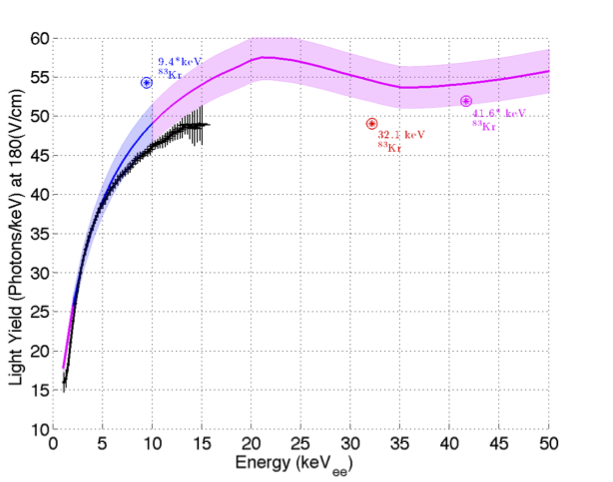
\includegraphics[width=80mm]{fig/LY_180_band_Tritium_Dec_2013_Charge_Yield_180_corr.png}
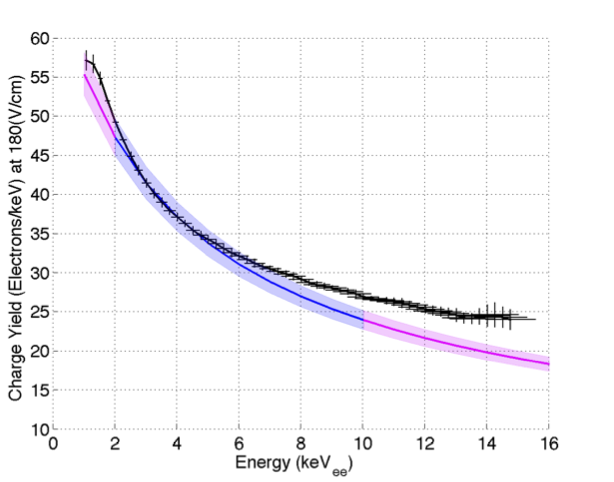
\includegraphics[width=80mm]{fig/QY_180_Tritium_Dec_2013_Charge_Yield_180_corr.png}
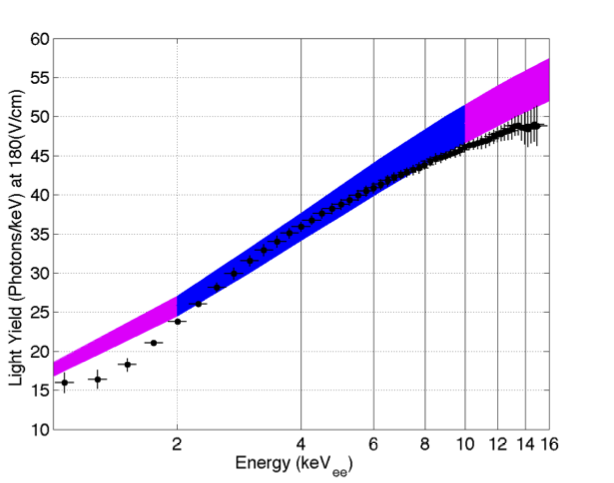
\includegraphics[width=83mm]{fig/LY_180_band_log_Tritium_Dec_2013_Charge_Yield_180_corr.png}
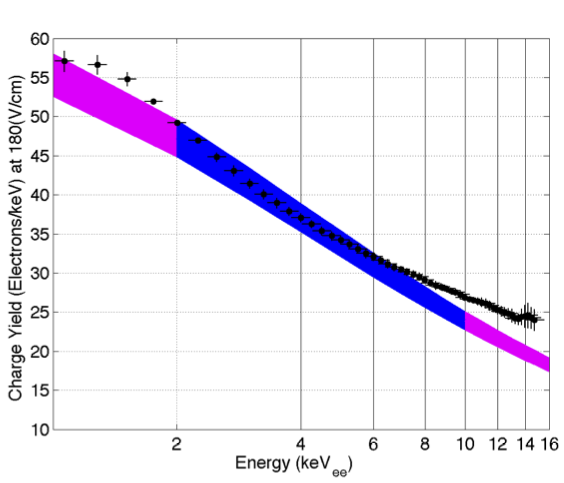
\includegraphics[width=76mm]{fig/QY_180_log_Tritium_Dec_2013_Charge_Yield_180_corr.png}
\caption{180 [V/cm], corrected for spectral shape. Top Left: Mean scintillation yield vs. combined energy using tritium beta decay (black line). $\rm^{83}Kr$ lines are plotted for reference but only the 32.1 [keV] line (red star) is kosher since the 9.4 [keV] line is dependent on timing separation, the 9.4 [keV] line is plotted (blue star) for separations greater than 1000 [ns]. Top Right: Mean ionization yield vs. combined energy (black line). Bottom Left: Scintillation yield vs. combined energy on a log scale. Bottom Right: Ionization yield vs. combined energy on a log scale. The shaded blue regions represent the NEST mean with $\pm 5\%$ that has been vetted by data [Erik Dahl Thesis]. The shaded magenta regions represent the NEST extrapolations from data. The measurement is made at a field of 180 [V/cm] and contains over 150,000 beta decays. The endpoint of the tritium beta spectrum is 18.6 [keV]}
\label{fig:L_Q_Yield_180}
\end{figure}




 \begin{figure}[h!]\centering
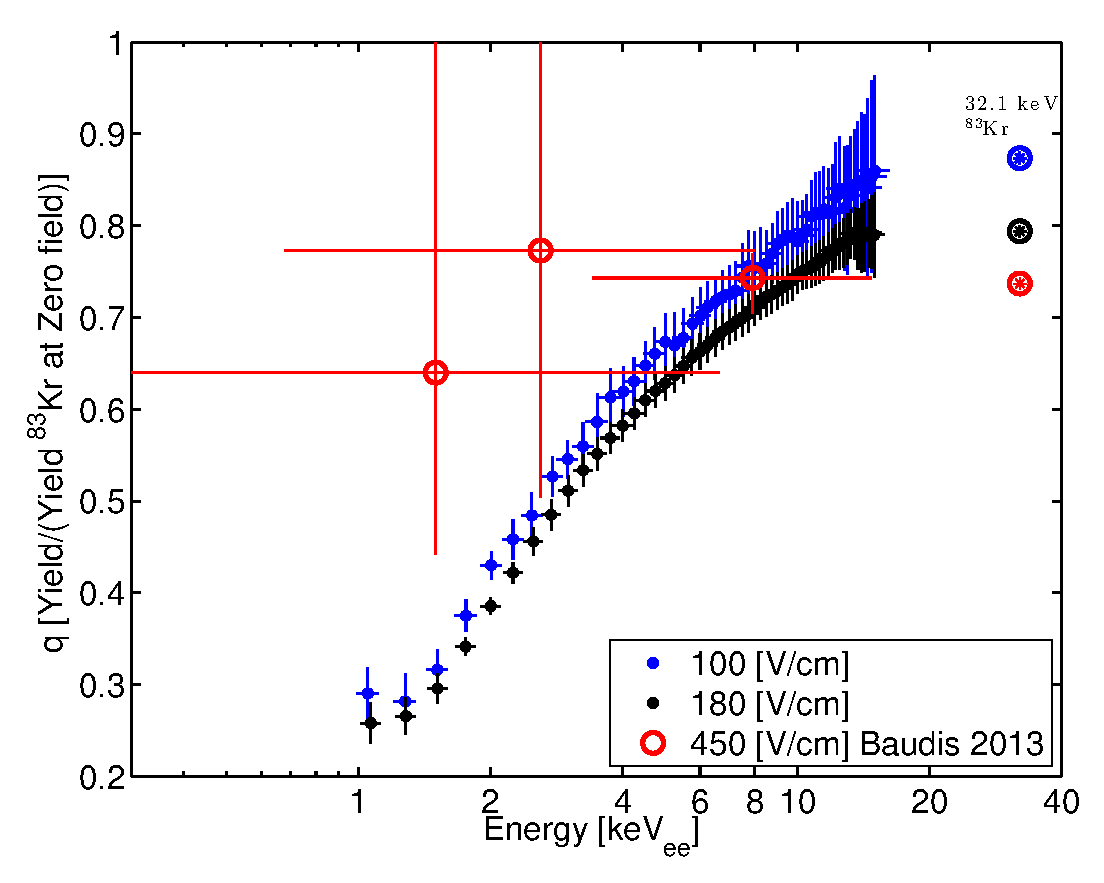
\includegraphics[width=100mm]{fig/q_all_log_Tritium_Dec_2013_Charge_Yield_180_corr.eps}
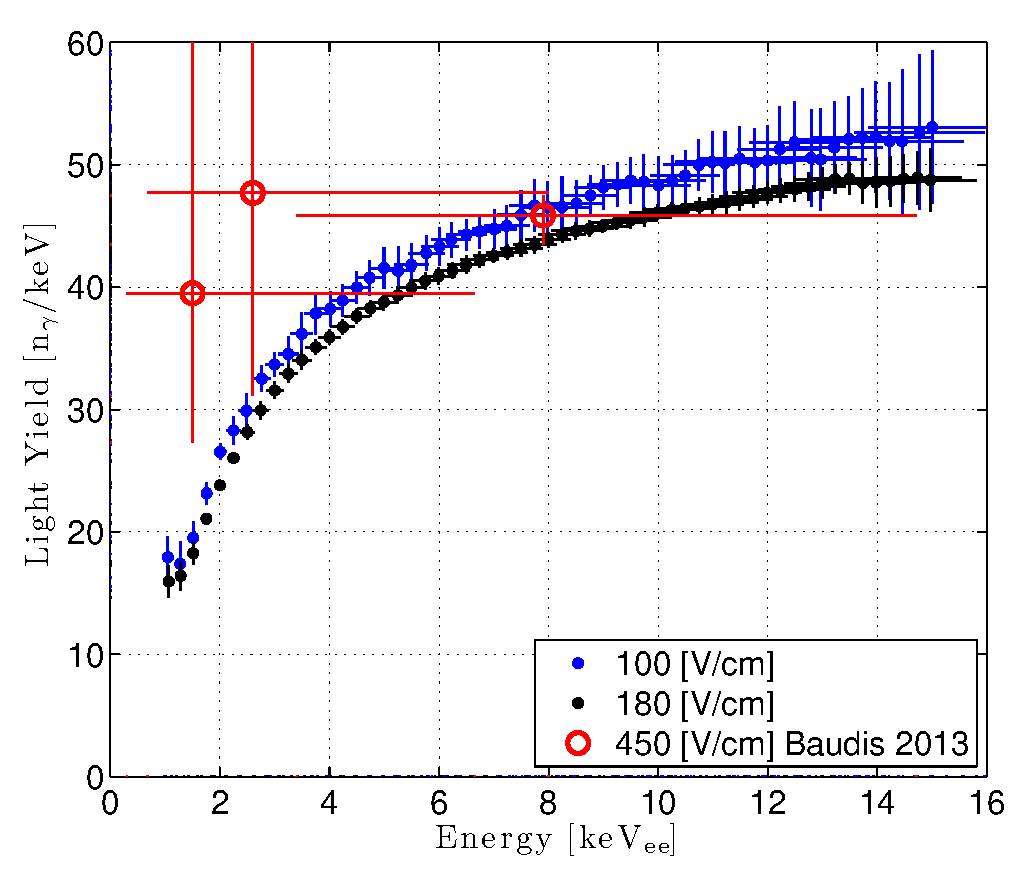
\includegraphics[width=82mm]{fig/LY_all_Tritium_Dec_2013_Charge_Yield_180_corr.eps}
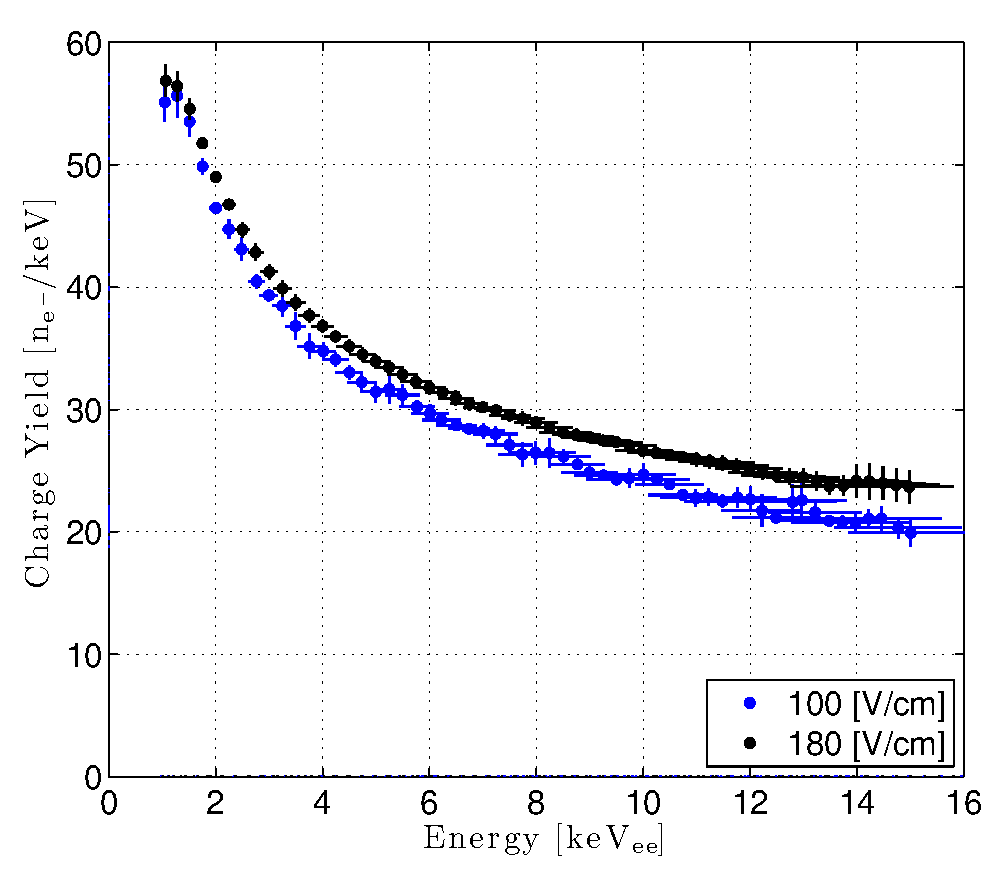
\includegraphics[width=80mm]{fig/Charge_Y_all_Tritium_Dec_2013_Charge_Yield_180_corr.eps}
\caption{Top: Scintillation yield relative to the yield of the 32.1 gamma of [keV] $\rm^{83}Kr $  vs. Energy. Shaded blue curve is tritium at 100 [V/cm], shaded black curve is tritium at 180 [V/cm], red points represent a recent Compton scattering measurement at 450 [V/cm]. Also shown are the corresponding quenching of the 32.1 [keV]  gamma of $\rm^{83}Kr$ (star inside circle). Bottom: scintillation yield [Photons/keV] vs. Energy. Shaded blue curve is tritium at 100 [V/cm], shaded black curve is tritium at 180 [V/cm], red circles represent a recent Compton scattering measurement at 450 [V/cm].}
\label{fig:L_Q_Yield_Baudis}
\end{figure}



\end{comment}
%%%%%%%%%%%%%%%%%%%%%%%%%%%%%%%%%%%%%%%%%%%%%%%%%%%%%%%%%%

\section{Additional Calibrations with Tritium}

In this paper we have described the development and use of a CH$_3$T calibration source for large scale xenon detectors. The primary application of the CH$_3$T calibration source is to characterize the ER band and measure discrimination from electronic and nuclear recoils. However, much more fundamental xenon physics can be probed with the CH$_3$T calibration source. With higher statistics the discrimination can be measured in finer bins of energy or S1 Phe (figure \ref{fig:Leak}) along with the Gaussianity of the ER band. The log(S2/S1) has been assumed to have Gaussian behavior in past experiments, never before has there been an ER calibration with such high data purity in the WIMP search region to observe potential non-Gaussian behavior. The largest CH$_3$T calibration in LUX detector's fiducial region produced 115,000 CH$_3$T beta decays with only three being non CH$_3$T events. 
The CH$_3$T calibration can also used to calculate the light yield, charge yield and recombination fluctuation over the range from 1 to 18 $\rm KeV_{ee}$. The current data taken with the LUX detector has allowed for the vetting of the NEST model down to 1 $\rm keV_{ee}$ for the first time. Finally, CH$_3$T provides a low energy uniformly distributed source making it ideal for determining the fiducial volume of a detector and calibrating position reconstruction algorithms for low energy events.


